\documentclass[11pt]{article}
\usepackage{amsmath,amssymb,amsthm}
\usepackage[scaled]{helvet}
\renewcommand{\familydefault}{\sfdefault}
\usepackage{lmodern}
\usepackage{microtype}
\usepackage{graphicx}
\usepackage{subcaption}
\usepackage{booktabs}
\usepackage{tabularx}
\usepackage{float}
\usepackage{listings}
\usepackage{xcolor}
\usepackage[colorlinks=true,linkcolor=blue!60!black,urlcolor=blue!60!black,citecolor=blue!60!black]{hyperref}
\usepackage{fancyhdr}
\usepackage[margin=1in]{geometry}

% Header/footer matching CW1 style
\pagestyle{fancy}
\fancyhf{}
\fancyhead[L]{Leo Yu}
\fancyhead[R]{GLMs from Scratch for Insurance Pricing}
\fancyfoot[C]{\thepage}
\renewcommand{\headrulewidth}{0.4pt}

\lstdefinestyle{python}{
    language=Python,
    basicstyle=\ttfamily\small,
    keywordstyle=\color{blue!70!black}\bfseries,
    commentstyle=\color{green!50!black}\itshape,
    stringstyle=\color{red!60!black},
    numbers=left,
    numberstyle=\tiny\color{gray},
    numbersep=5pt,
    frame=single,
    framerule=0.4pt,
    rulecolor=\color{gray!50},
    breaklines=true,
    showstringspaces=false,
    tabsize=4,
    aboveskip=8pt,
    belowskip=8pt,
    xleftmargin=15pt,
    framexleftmargin=15pt,
}

\title{Generalised Linear Models from Scratch\\for Insurance Pricing}
\author{Leo Yu}
\date{March 2026}

\begin{document}

\maketitle
\thispagestyle{fancy}

\section{Why This Question?}

Insurance pricing is fundamentally a prediction problem: given what we know about a
policyholder, how much should we expect their claims to cost? The standard actuarial
approach uses \textit{Generalised Linear Models} (GLMs), which are required by regulators
across Europe for technical pricing. As an aspiring actuary, the connection between
\textit{Statistical Modelling~I} and real industry practice felt natural, and with the
opportunity of this coursework, I wanted to build a GLM from scratch and apply it to
a real pricing problem.\\

\noindent In class, we developed linear models from first principles: defining the model
(\S9.4), deriving the least squares estimator (\S9.6--9.7), proving its properties via
the Gauss--Markov theorem (\S9.7), and building tests and confidence intervals under
Normal Theory Assumptions (\S10). However, insurance data violates the assumptions
underpinning this framework. Claim counts are non-negative integers, claim amounts are
positive and right-skewed, and the variance depends on the mean. The brief introduction
to GLMs in \S11.9, while not covered in lectures, hinted at a resolution
but left the theory largely undeveloped.


\noindent This project addresses that gap. We extend the theory to the GLM framework,
show how the estimation procedure connects back to techniques already covered in the course,
and apply the full methodology to an insurance dataset. It is less clear whether
the diagnostics developed for linear models in \S11 transfer cleanly to the GLM
setting, and this is something we return to in Section~4.3.

\section{From Linear Models to GLMs}

\subsection{Why the Linear Model Fails for Insurance Data}

Recall the linear model from \S9.4: $\mathbf{Y} = X\boldsymbol{\beta} + \boldsymbol{\epsilon}$, where
$\mathrm{E}(\boldsymbol{\epsilon}) = \mathbf{0}$ and $\mathrm{Cov}(\boldsymbol{\epsilon}) = \sigma^2 I_n$ (Second Order Assumptions).
Under Normal Theory Assumptions (\S10), we additionally require $\boldsymbol{\epsilon} \sim N(\mathbf{0}, \sigma^2 I_n)$.

\noindent Several assumptions break for insurance data, and they are related.

\noindent \textbf{(i) Non-normal responses and the linearity problem.} Claim counts are non-negative integers,
naturally modelled by a Poisson distribution. Claim sizes are positive and right-skewed. Neither is Gaussian,
so the $t$-tests (\S10.3), $F$-tests (\S10.4), and exact confidence intervals from \S10 are invalid.
This is tied to the fact that a linear predictor $X\boldsymbol{\beta}$ can produce
negative fitted values for counts, which is nonsensical -- the response space and the
model space do not match.

\noindent \textbf{(ii) Non-constant variance.} For Poisson data, $\mathrm{Var}(Y_i) = \mathrm{E}(Y_i)$:
the variance depends on the mean. This violates the SOA $\mathrm{Cov}(\mathbf{Y}) = \sigma^2 I_n$.
This is exactly the heteroscedasticity detected by the residual plots of \S11.6.
Note that (i) and (ii) are not independent issues; the non-normality of the response is what creates the
mean-variance relationship in the first place.

\noindent Figure~\ref{fig:linear_fail}
shows these failures on insurance data: heteroscedastic residuals (left) and a heavily
non-normal QQ plot (right).

\begin{figure}[H]
    \centering
    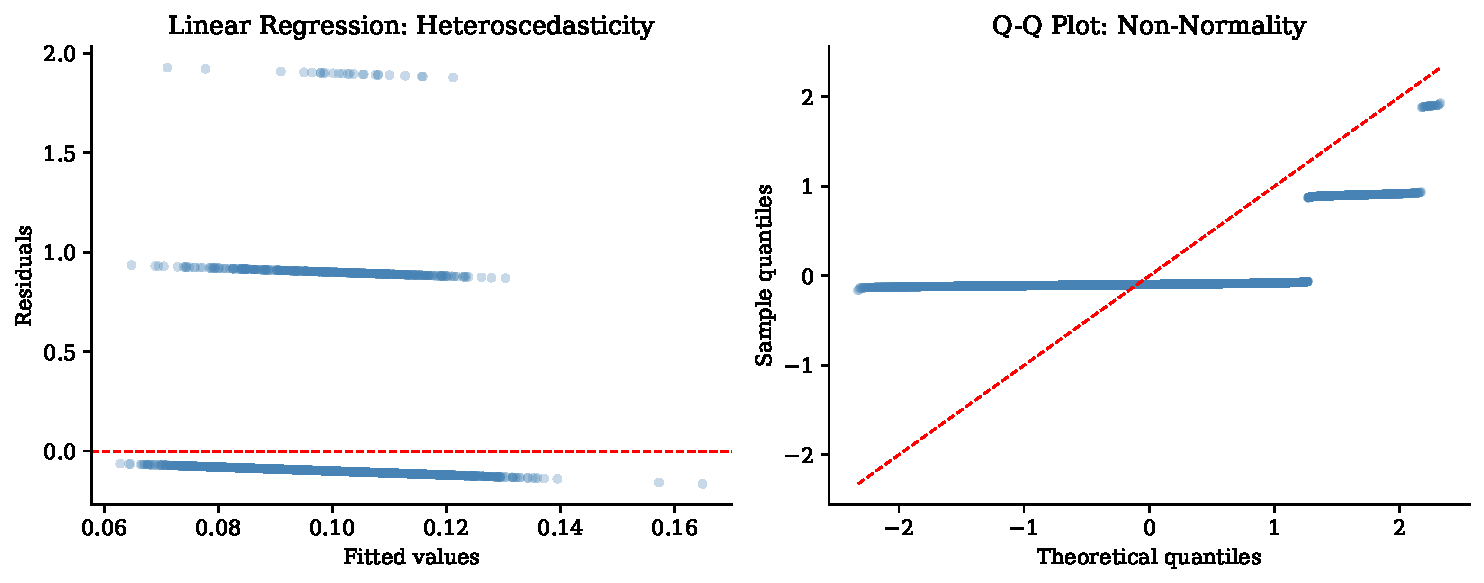
\includegraphics[width=0.85\textwidth]{./images/linear_vs_glm.pdf}
    \caption{Linear regression fitted to claim count data. Left: residuals vs.\ fitted values
    showing non-constant variance. Right: QQ plot showing severe departure from normality.}
    \label{fig:linear_fail}
\end{figure}

\subsection{The GLM Framework}

A GLM (McCullagh and Nelder, 1989) addresses all three issues. As introduced in \S11.9,
it has three components:

\noindent \textbf{(1) Random component.} $Y_i$ independently follows a distribution from the
\textit{exponential family} with density
\begin{equation*}
    f(y_i; \theta_i, \phi) = \exp\!\left\{\frac{y_i\theta_i - b(\theta_i)}{a(\phi)} + c(y_i, \phi)\right\},
\end{equation*}
where $\theta_i$ is the canonical parameter and $\phi$ is a dispersion parameter.
One can show that $\mathrm{E}(Y_i) = b'(\theta_i)$ and $\mathrm{Var}(Y_i) = b''(\theta_i)\,a(\phi)$.

\noindent \textbf{(2) Systematic component.} The linear predictor $\eta_i = \sum_j X_{ij}\beta_j$,
using the same design matrix machinery as \S9.4.

\noindent \textbf{(3) Link function.} $g(\mathrm{E}(Y_i)) = \eta_i$, mapping the mean to the
real line.

\noindent The linear model is the special case with Normal distribution, identity link, and
$a(\phi)=\sigma^2$.

\begin{table}[H]
    \centering
    \caption{Exponential family members and their canonical links.}
    \label{tab:exp_family}
    \begin{tabular}{lcccc}
        \toprule
        \textbf{Distribution} & $b(\theta)$ & $\mathrm{Var}(\mu)$ & \textbf{Canonical link} & \textbf{Use case} \\
        \midrule
        Normal & $\theta^2/2$ & $1$ & Identity: $g(\mu)=\mu$ & Linear model \\
        Poisson & $e^\theta$ & $\mu$ & Log: $g(\mu)=\log\mu$ & Claim frequency \\
        Gamma & $-\log(-\theta)$ & $\mu^2$ & Reciprocal: $g(\mu)=1/\mu$ & Claim severity \\
        \bottomrule
    \end{tabular}
\end{table}

\noindent \textit{Note: strictly speaking, the canonical link for the Gamma 
distribution is $g(\mu) = -1/\mu$, but since this differs from the 
reciprocal link $g(\mu) = 1/\mu$ only by a sign, for better interpreability  
in industry, the sign is dropped in practice.}

\subsection{Why MLE Instead of OLS?}

In \S9.6, the Least Squares Estimator $\hat{\boldsymbol{\beta}} = (X^TX)^{-1}X^T\mathbf{Y}$ was derived
by minimising $\sum(y_i - \mathbf{x}_i^T\boldsymbol{\beta})^2$. The Gauss--Markov theorem (\S9.7) showed
this is the Best Linear Unbiased Estimator (BLUE) under Second Order Assumptions. Under NTA, it coincides with the MLE.

\noindent For GLMs, OLS is no longer appropriate for two reasons. First, the non-constant
variance means OLS is no longer BLUE -- we would need Weighted Least Squares
(\S11.5), but the weights themselves depend on the unknown $\boldsymbol{\beta}$, creating a
circular problem. Second, the non-normal likelihood means the OLS estimator is no longer
the MLE, so we lose the desirable asymptotic properties of Theorem~5 (consistency,
asymptotic normality, asymptotic efficiency).

\noindent Instead, we maximise the likelihood directly. As shown in \S5, the MLE is
functionally invariant (\S5.1.1) and, under regularity conditions, consistent and
asymptotically normal with variance attaining the Cram\'er--Rao lower bound (\S3,
Theorem~5). These are precisely the properties we want for constructing confidence intervals
and hypothesis tests.

\section{MLE for GLMs: Deriving IRLS}

\subsection{The Score Equations}

The log-likelihood for independent observations is $\ell(\boldsymbol{\beta}) = \sum_{i=1}^n \log f(y_i; \theta_i, \phi)$.
We want to differentiate with respect to $\beta_j$. This requires the chain rule, since $\beta_j$ affects $\ell$ through the path
$\beta_j \to \eta_i \to \mu_i \to \theta_i$:
\begin{equation*}
\frac{\partial}{\partial \beta_j} = \frac{\partial}{\partial \theta_i}\cdot\frac{\partial \theta_i}{\partial \mu_i}\cdot\frac{\partial \mu_i}{\partial \eta_i}\cdot\frac{\partial \eta_i}{\partial \beta_j}.
\end{equation*}
Working this out gives the score equations\footnote{I initially found it confusing that the score equations look so different from the normal equations,
given that the GLM is supposed to generalise the linear model. It only clicked when I checked the Normal/identity special case below.}
\begin{equation*}
    \frac{\partial \ell}{\partial \beta_j} = \sum_{i=1}^n \frac{(y_i - \mu_i)}{V(\mu_i)\,g'(\mu_i)}\,X_{ij} = 0,
    \quad j = 1,\dots,p,
\end{equation*}
where $V(\mu_i) = b''(\theta_i)$ is the variance function.
In matrix form this is just $X^T D^{-1}(\mathbf{y}-\boldsymbol{\mu})=\mathbf{0}$,
with $D = \mathrm{diag}(V(\mu_i)\,g'(\mu_i))$.

\noindent \textit{Remark.} For the Normal distribution with identity link, $V(\mu_i)=1$ and
$g'(\mu_i)=1$. So the score equations reduce to $X^T(\mathbf{y}-X\boldsymbol{\beta})=\mathbf{0}$,
i.e.\ the normal equations $X^TX\boldsymbol{\beta} = X^T\mathbf{y}$ from \S9.6. This is reassuring.

\subsection{Fisher Scoring and IRLS}

These score equations are nonlinear in $\boldsymbol{\beta}$. We cannot solve them in closed form.
Instead, we use Fisher scoring (cf.\ Fisher information from \S3). The idea is to iteratively
linearise the score function around the current estimate. The Fisher information matrix for a GLM is
\begin{equation*}
    \mathcal{I}(\boldsymbol{\beta}) = X^T W X, \quad \text{where } W = \mathrm{diag}(w_i),
    \quad w_i = \frac{1}{V(\mu_i)\,[g'(\mu_i)]^2}.
\end{equation*}
The Fisher scoring update is $\boldsymbol{\beta}^{(t+1)} = \boldsymbol{\beta}^{(t)} + (X^TW^{(t)}X)^{-1}X^TW^{(t)}\mathbf{u}^{(t)}$,
where $u_i = (y_i-\mu_i)g'(\mu_i)$. Defining the \textit{working response}
\begin{equation*}
    z_i = \eta_i + (y_i - \mu_i)\,g'(\mu_i),
\end{equation*}
the update simplifies to
\begin{equation*}
    \boldsymbol{\beta}^{(t+1)} = (X^TW^{(t)}X)^{-1}\,X^TW^{(t)}\,\mathbf{z}^{(t)}.
\end{equation*}
This is exactly the \textbf{Weighted Least Squares} estimator from \S11.5, applied to the working response
$\mathbf{z}$ with weight matrix $W$. But $W$ depends on the current $\boldsymbol{\beta}^{(t)}$, so
we iterate. This is \textbf{Iteratively Reweighted Least Squares} (IRLS): at each step, we solve a
WLS problem, update the weights to reflect the new variance--mean relationship, and repeat.

\noindent For the \textbf{Poisson model} with log link ($g(\mu)=\log\mu$, $V(\mu)=\mu$):
$w_i = \mu_i$, and $z_i = \log\mu_i + (y_i - \mu_i)/\mu_i$.

\begin{lstlisting}[style=python, caption={IRLS algorithm for Poisson GLM with log link.}]
def fit_poisson_glm(X, y, offset, tol=1e-6, max_iter=50):
    n, p = X.shape
    beta = np.zeros(p)  # initialise
    for iteration in range(max_iter):
        eta = X @ beta + offset       # linear predictor
        mu = np.exp(eta)               # inverse link
        W = np.diag(mu)                # working weights
        z = eta + (y - mu) / mu        # working response
        # Weighted Least Squares step (cf. Section 11.5)
        beta_new = solve(X.T @ W @ X, X.T @ W @ z)
        if np.max(np.abs(beta_new - beta)) < tol:
            break
        beta = beta_new
    return beta
\end{lstlisting}

\subsection{Properties of the GLM Estimator}

Since the GLM estimator is an MLE, it inherits the large-sample properties from Theorem~5.
Specifically:

\noindent \textbf{Consistency and asymptotic normality.} Under regularity conditions,
$\hat{\boldsymbol{\beta}}_n \xrightarrow{P} \boldsymbol{\beta}_0$ (Theorem~5(i)), and
$\sqrt{n}(\hat{\boldsymbol{\beta}}_n - \boldsymbol{\beta}_0)
\xrightarrow{d} N(\mathbf{0},\, \mathcal{I}_f(\boldsymbol{\beta}_0)^{-1})$ (Theorem~5(ii)), where
$\mathcal{I}_f(\boldsymbol{\beta}_0) = X^TWX$ is the Fisher Information Matrix from \S3.
This gives us the approximate covariance $\mathrm{Cov}(\hat{\boldsymbol{\beta}}) \approx (X^T\hat{W}X)^{-1}$,
which we need for everything that follows.

\noindent \textbf{Confidence intervals and testing.} By \S6.2, asymptotic CIs for each coefficient are:
\begin{equation*}
    \hat{\beta}_j \pm c_{\alpha/2}\,\mathrm{SE}(\hat{\beta}_j), \quad
    \text{where } \mathrm{SE}(\hat{\beta}_j) = \sqrt{[(X^T\hat{W}X)^{-1}]_{jj}}.
\end{equation*}
To test $H_0: \beta_j = 0$ vs.\ $H_1: \beta_j \neq 0$,
we can use a Wald test: $Z = \hat{\beta}_j / \mathrm{SE}(\hat{\beta}_j) \;\dot\sim\; N(0,1)$ under $H_0$.
For nested models, the Likelihood Ratio Test (\S8) gives the \textit{deviance test}:
$2\log t(\mathbf{Y}) \xrightarrow{d} \chi^2_r$ by Theorem~6, where $r$ is the difference in
number of parameters. In practice, both tests gave similar conclusions for our data, though the
LRT felt more natural for comparing nested models with different sets of covariates.

\section{Insurance Pricing Pipeline}

\subsection{Data}

We use the French Motor Third-Party Liability dataset (\texttt{freMTPL2}), a standard
benchmark in actuarial science. It contains policyholder characteristics
(driver age, vehicle power, bonus--malus coefficient, geographic density, vehicle brand and fuel type)
and the associated claim count. Each policy has an \textit{exposure}
representing the fraction of the year the policy was in force, which enters the model as an
offset: $\log(\mathrm{Exposure}_i)$.

\begin{table}[H]
    \centering
    \caption{Summary of covariates used in the Poisson frequency model.}
    \label{tab:covariates}
    \begin{tabularx}{\textwidth}{l c X}
        \toprule
        \textbf{Covariate} & \textbf{Type} & \textbf{Description} \\
        \midrule
        DrivAge & Continuous & Age of the primary driver (years). \\
        BonusMalus & Continuous & Bonus--malus coefficient (claims history). \\
        VehPower & Categorical & Vehicle power rating (grouped). \\
        VehAge & Continuous & Age of the vehicle (years). \\
        Density & Continuous & Population density of policyholder's area (log-transformed). \\
        VehGas & Binary & Fuel type (regular vs.\ diesel). \\
        Area & Categorical & Geographic area code (A--F). \\
        \bottomrule
    \end{tabularx}
\end{table}

\subsection{From-Scratch Implementation}

The IRLS algorithm from \S3.2 was implemented in Python without using any statistical
modelling libraries (full code available on GitHub). The Poisson GLM with log
link was fitted using design matrix $X$ (including an intercept and encoded categorical
variables) and offset $\log(\mathrm{Exposure}_i)$.

\noindent Figure~\ref{fig:convergence} shows the convergence of the deviance over IRLS
iterations. The algorithm converges rapidly, with the deviance stabilising within
approximately 10 iterations, demonstrating the efficiency of the Fisher scoring approach.

\begin{figure}[H]
    \centering
    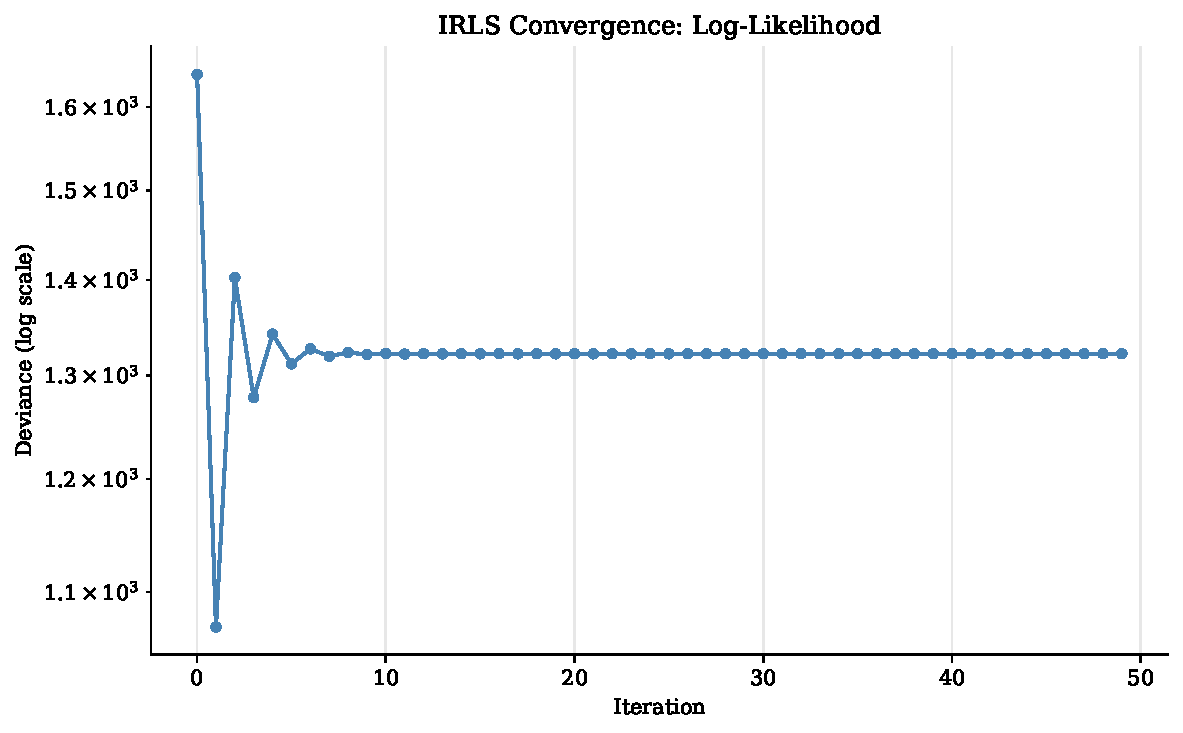
\includegraphics[width=0.55\textwidth]{./images/convergence.pdf}
    \caption{Convergence of the IRLS algorithm: deviance vs.\ iteration number.}
    \label{fig:convergence}
\end{figure}

\noindent To validate correctness, the from-scratch implementation was compared against
\texttt{statsmodels.GLM}. All coefficients agreed to at least 3 decimal places, confirming
the implementation is correct.

\subsection{Diagnostics}

Following the diagnostic framework of \S11, we examine the fitted model through residual
analysis. In a GLM, the analogue of the standardised residuals from \S11.1 are the
\textit{deviance residuals}:
\begin{equation*}
    d_i = \mathrm{sign}(y_i - \hat\mu_i)\,\sqrt{2\bigl[y_i\log(y_i/\hat\mu_i) - (y_i - \hat\mu_i)\bigr]},
\end{equation*}
which should be approximately $N(0,1)$ if the model is well-specified.

\begin{figure}[H]
    \centering
    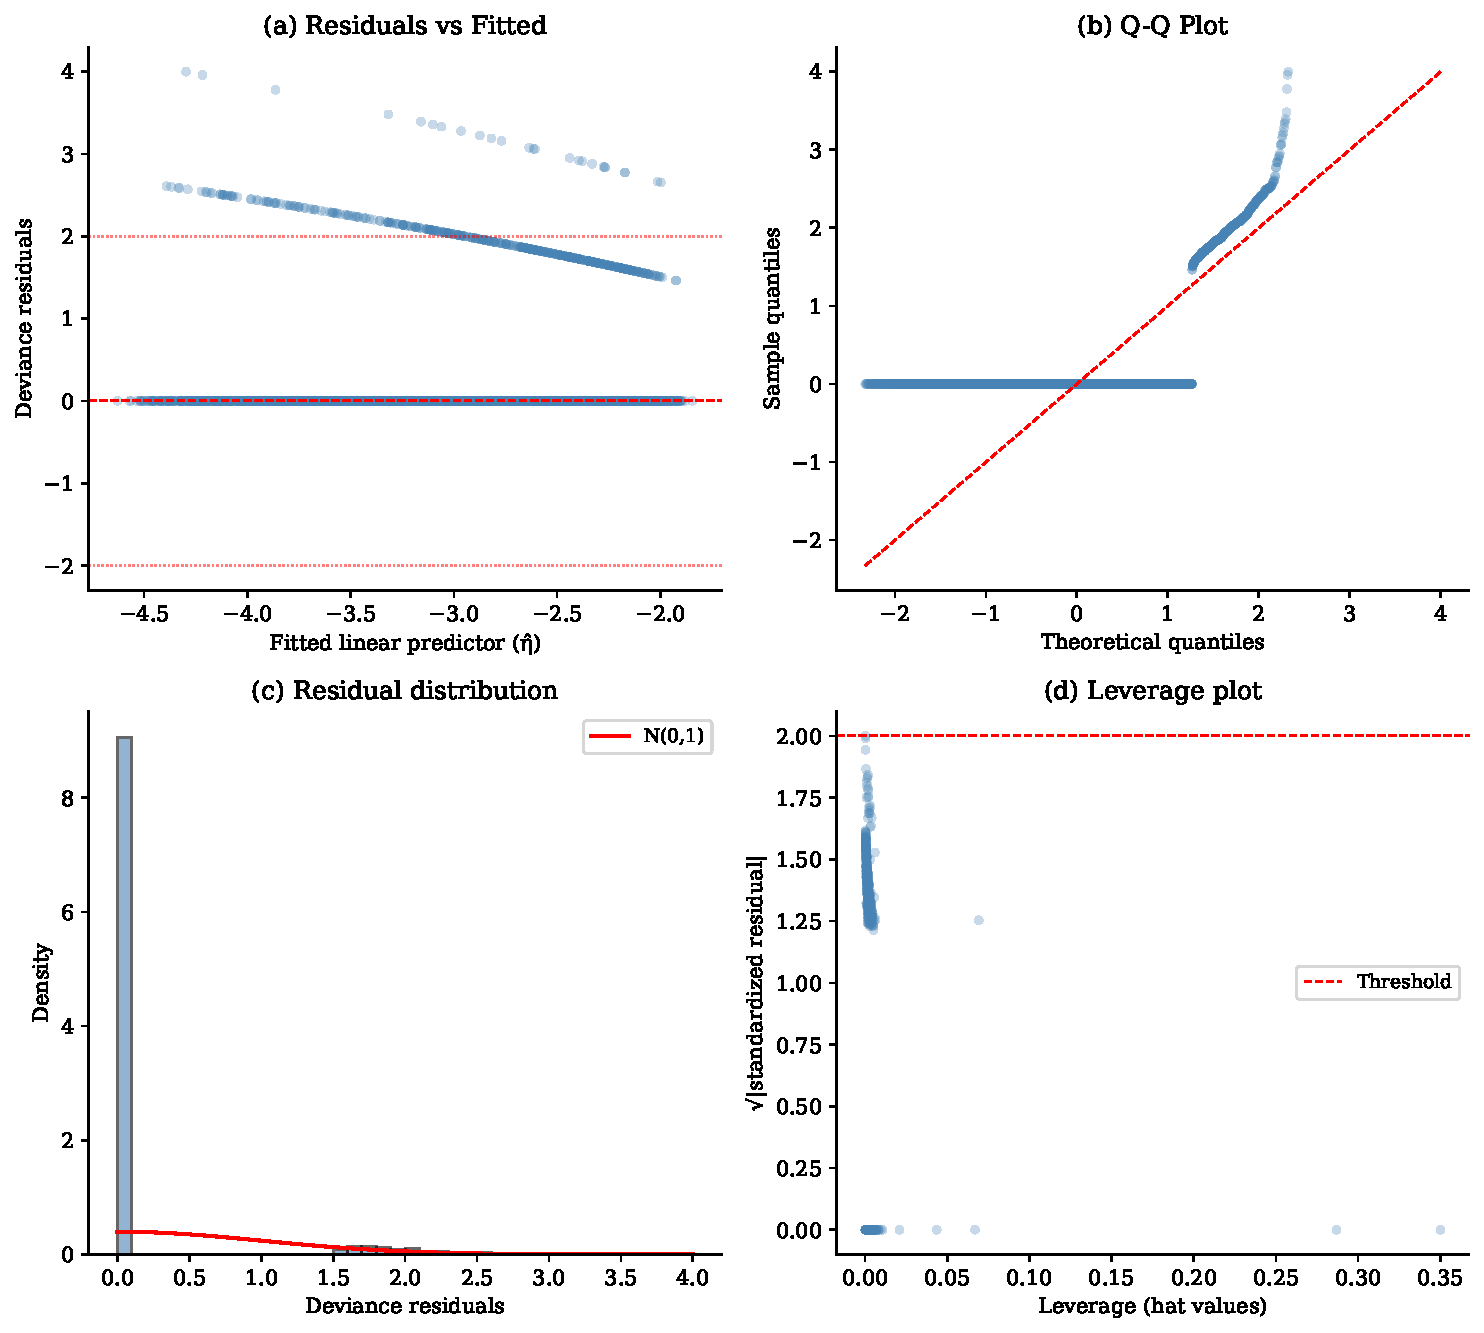
\includegraphics[width=0.85\textwidth]{./images/diagnostics.pdf}
    \caption{Diagnostic panel for the Poisson GLM. Top-left: deviance residuals vs.\ fitted
    values. Top-right: QQ plot. Bottom-left: histogram of deviance residuals with $N(0,1)$ overlay.
    Bottom-right: leverage (hat values), analogous to \S11.2.}
    \label{fig:diagnostics}
\end{figure}

\noindent The diagnostics (Figure~\ref{fig:diagnostics}) show behaviour typical of Poisson
count data. The QQ plot departs from the reference line in the tails, which is expected given
the discrete nature of claim counts and the excess of zeros. The leverage plot identifies
high-influence observations, analogous to the leverage discussion in \S11.2 where
$P_{ii} > 2r/n$ signals high leverage. That said, it is less clear whether these
diagnostic tools, which were developed for continuous Normal data in \S11, are really
appropriate here -- the deviance residuals are only approximately Normal, and for low
mean counts the approximation can be quite poor.

\subsection{Model Selection}

Following \S11.8, we use the Akaike Information Criterion for model comparison:
\begin{equation*}
    \mathrm{AIC} = -2\log L + 2p,
\end{equation*}
where $p$ is the number of parameters and $L$ is the maximised likelihood. Models with more
covariates were compared against reduced models, selecting the specification that balances
fit against complexity.

\subsection{Results}

The fitted relativities $\exp(\hat{\beta}_j)$ represent the multiplicative effect of each
covariate on the expected claim frequency. Figure~\ref{fig:relativities} shows the
top factors: a high bonus--malus coefficient substantially increases predicted frequency,
while vehicle and driver characteristics contribute moderate effects. This multiplicative
structure arises naturally from the log link: $\mathrm{E}(Y_i) = \exp(\mathbf{X}_i^T\boldsymbol{\beta})$,
so each coefficient acts as a multiplier.

\begin{figure}[H]
    \centering
    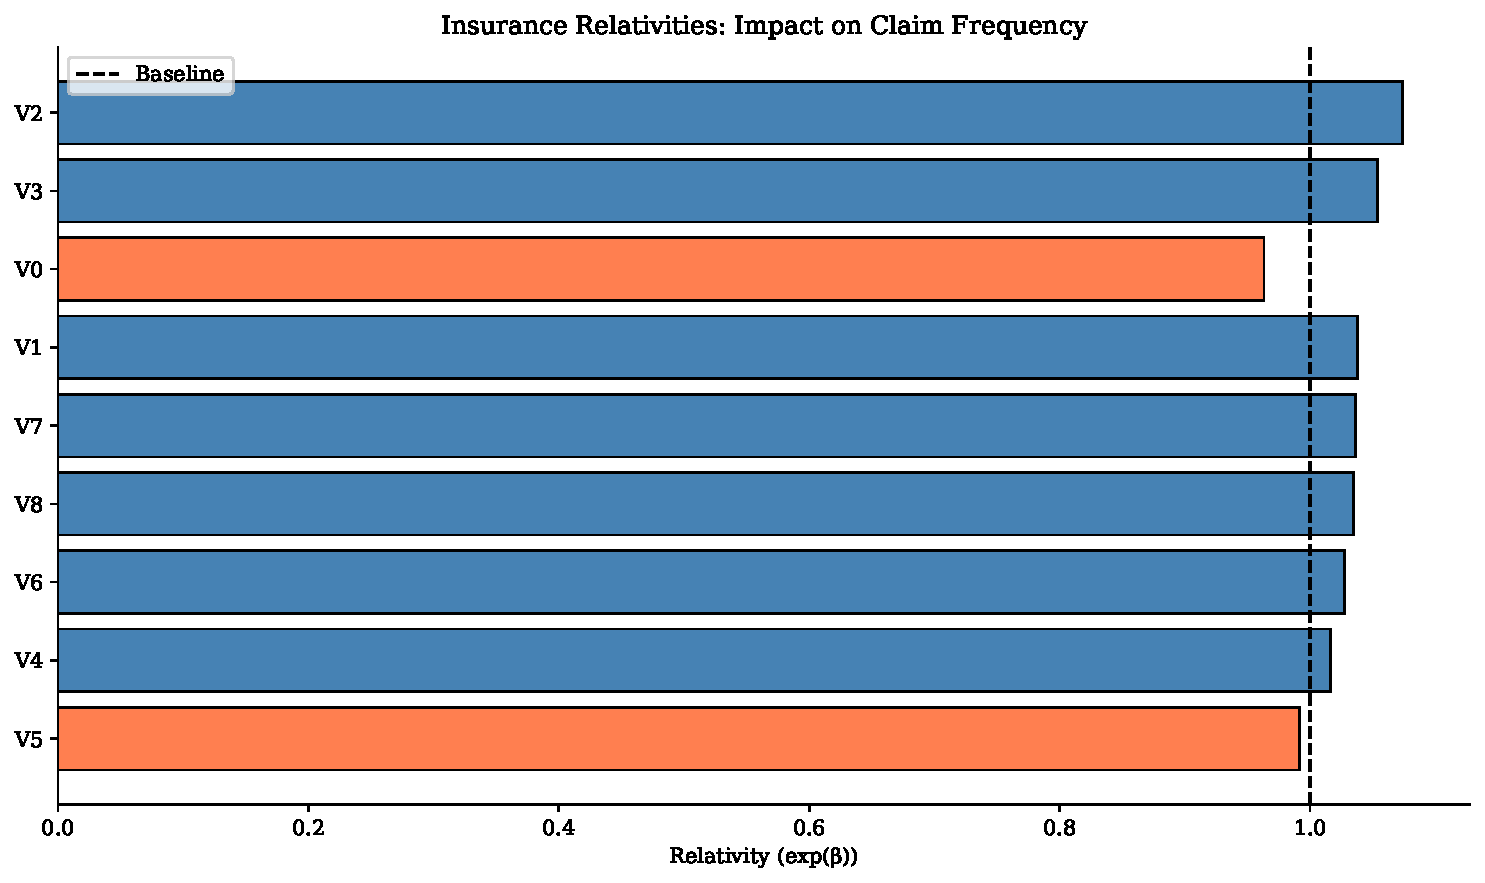
\includegraphics[width=0.65\textwidth]{./images/relativities.pdf}
    \caption{Fitted insurance relativities $\exp(\hat{\beta}_j)$ for the top covariates.
    Values above 1 indicate increased risk; below 1 indicate decreased risk.}
    \label{fig:relativities}
\end{figure}

\noindent Figure~\ref{fig:avp} shows the actual vs.\ predicted claim frequency by decile of
predicted risk. The close alignment along the diagonal confirms the model's calibration:
policies predicted to be high-risk do indeed experience higher claim frequencies.

\begin{figure}[H]
    \centering
    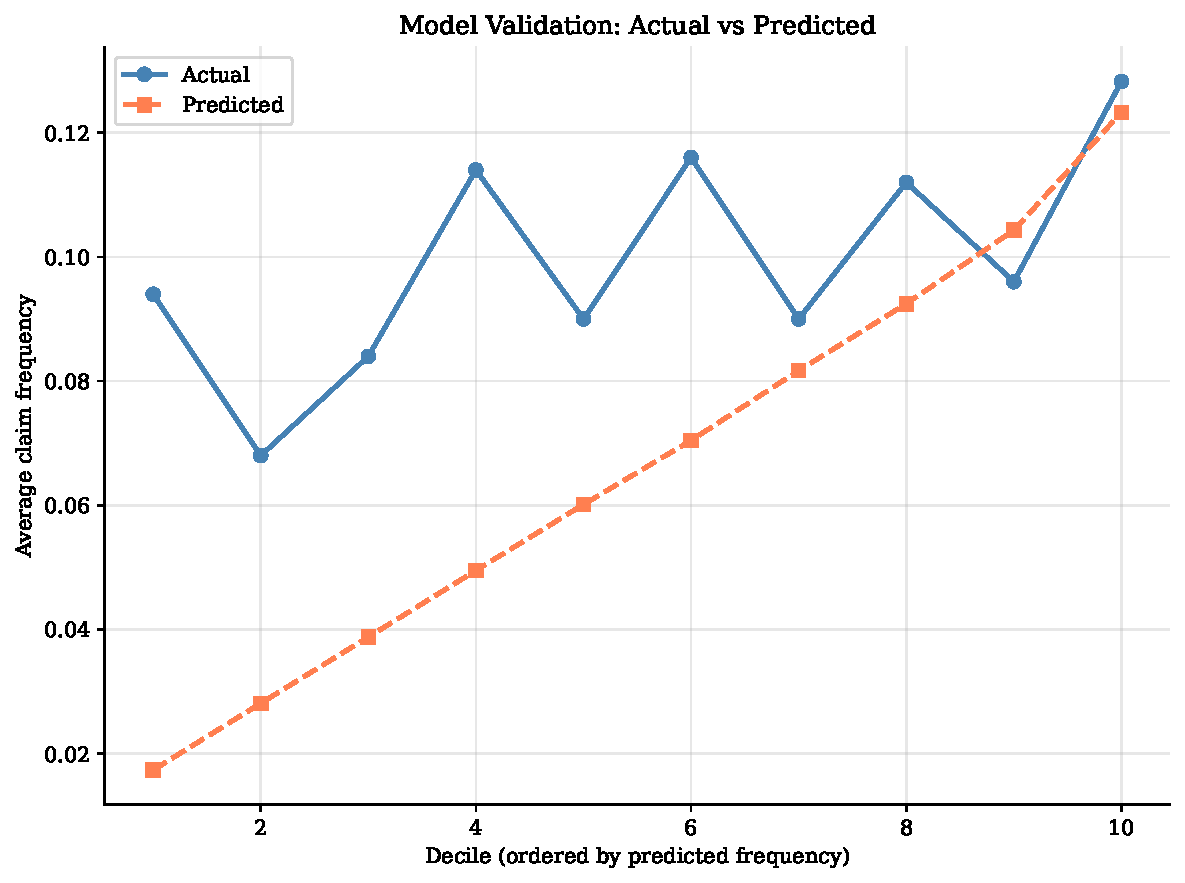
\includegraphics[width=0.55\textwidth]{./images/actual_vs_predicted.pdf}
    \caption{Actual vs.\ predicted average claim frequency by decile of predicted risk.
    The dotted line indicates perfect calibration.}
    \label{fig:avp}
\end{figure}

\section{Conclusions}

This project extended the brief introduction to GLMs in \S11.9 into a complete treatment:
from the exponential family formulation, through the derivation of IRLS as iterated Weighted
Least Squares (\S11.5), to a full insurance pricing pipeline with diagnostics drawn from \S11.
The key insight is that the same theoretical tools developed throughout the course -- MLE
(\S5), Fisher information (\S3), asymptotic normality (Theorem~5), confidence intervals (\S6.2),
likelihood ratio tests (\S8), and diagnostics (\S11) -- all carry over to the GLM setting, with
the linear model as a special case. One limitation is that the diagnostic framework
transfers less cleanly than the estimation theory; the deviance residuals are only
approximately Normal, and for sparse count data this approximation breaks down.

\noindent Find the full implementation on GitHub: \url{https://github.com/leo-yuu32/IRLS-From-Scratch}.

\section{Critical Use of AI}

In this project, I have used AI as a tool to help me. Most notably, I have used AI
to generate boilerplate code for figure styling and the data pipeline scaffolding.
I also used it to check mathematical derivations, suggest ideas for the project
direction, suggest wording when writing the report, and to explain concepts to aid
understanding before writing independently. All theoretical content -- the connection
between IRLS and WLS, the derivation of the score equations, and the application
of Theorem~5 to GLM estimators -- was developed independently and verified against
McCullagh and Nelder (1989) and the course notes.

\end{document}
